\documentclass[11pt,fleqn]{exam}
\usepackage[utf8]{inputenc}
\usepackage[T1]{fontenc}
\usepackage{fancyvrb}
\usepackage{amsmath}
\usepackage{amssymb}
\usepackage{hyperref}
\usepackage{algpseudocode}
\usepackage{comment}
\usepackage{enumitem}
\usepackage[margin=0.75in]{geometry}
\usepackage{tikz}
\usetikzlibrary{arrows,arrows.meta,positioning,intersections,shapes.gates.logic.US,calc}
\algnewcommand\algorithmicforeach{\textbf{for each}}
\algdef{S}[FOR]{ForEach}[1]{\algorithmicforeach\ #1\ \algorithmicdo}
\newcommand{\fillinMCmath}[1]{
\begin{tikzpicture}\draw circle [radius=0.5em];\end{tikzpicture}\ #1}
\newcommand{\fillinMCmathsoln}[1]{
\begin{tikzpicture}\draw[black, fill=blue] circle [radius=0.5em];\end{tikzpicture}\ #1}
\newcommand{\fillinblank}[1]{\fillinblankmath{\mbox{#1}}}
\newcommand{\fillinblankmath}[1]{\begingroup\setlength{\fboxsep}{1em}\setlength{\fboxrule}
{2pt}\fbox{\LARGE\phantom{#1}}\endgroup}
\newcommand{\fillinblankmathsoln}[1]{\begingroup\setlength{\fboxsep}{1em}\setlength{\fboxrule}
{2pt}\fbox{#1}\endgroup}
\newcommand{\ptsamt}[1]{[#1~points]}
\newcommand{\ptamt}[1]{[#1~point]}

%%% Adding Colour to Questions and Answers
\usepackage{color}

\definecolor{solnblue}{rgb}{0,0,1}
\newenvironment{soln}{\color{solnblue}}{}

%fancyvrb commands
\def\lar{$\leftarrow$}
\def\lesseq{$\leq$}
\def\alp{$\alpha$}
\def\inf{$\infty$}

%Questions

% Answers
\definecolor{blu}{rgb}{0,0,0.5}
\def\blu#1{{\color{blu}#1}}
\definecolor{gre}{rgb}{0,.3,0}
\def\gre#1{{\color{gre}#1}}
\definecolor{red}{rgb}{0.5,0.0,0}
\def\red#1{{\color{red}#1}}
\def\norm#1{\|#1\|}
%%% End for Colours

\bracketedpoints

\makeatletter
\renewenvironment{solution}{\leavevmode\par\begin{soln}\noindent Solution:}{\end{soln}}
\makeatother


\title{CPSC 320 2024W1: Assignment 4}
	
\author{}
\date{}

\title{CPSC 320 2024W1: Assignment 5}

\begin{document}

	\maketitle

 This assignment is due \textbf{Friday, December 6 at 7 PM}. Late submissions will not be accepted. All the submission and formatting rules for Assignment~1 apply to this assignment as well.  

%------------------------------------------------------------------------------------
\section{List of names of group members (as listed on Canvas)}

Provide the list here. This is worth 1 mark. Include student numbers as a secondary failsafe if you wish.

\section{Statement on collaboration and use of resources}
To develop good practices in doing homeworks, citing resources and acknowledging input from others, please complete the following. This question is worth 2 marks.

\begin{enumerate}
\item All group members have read and followed the guidelines for groupwork on assignments given in the Syllabus).

\fillinMCmath{Yes} \hspace{.5in} \fillinMCmath{No}

\item We used the following resources (list books, online sources, etc. that you consulted):
\item One or more of us consulted with course staff during office hours.

\fillinMCmath{Yes} \hspace{.5in} \fillinMCmath{No}

\item One or more of us collaborated with other CPSC 320 students; none of us took
      written notes during our consultations and we took at least a half-hour break afterwards.

\fillinMCmath{Yes} \hspace{.5in} \fillinMCmath{No}

      If yes, please list their name(s) here:

\item One or more of us collaborated with or consulted others outside of CPSC 320; none of us took written notes during our consultations and we took at least a half-hour break afterwards.

\fillinMCmath{Yes} \hspace{.5in} \fillinMCmath{No}

      If yes, please list their name(s) here:

\end{enumerate}

	\clearpage

%==========================================
    
\section{The Path To Victory 2.0}

A Hamiltonian Path is a path in a graph that visits each vertex exactly once. In this question, we consider the variant of the Hamiltonian Path problem with the start and end node specified: that is, given a graph $G=(V,E)$ and two nodes $s$ and $t$, does there exist a path from $s$ to $t$ that visits every node in $G$ exactly once? You can may assume that $G$ contains at least three vertices.

The Hamiltonian Path problem can be applied to graphs that are either undirected or directed. For example, the undirected graph below has a Hamiltonian Path from A to D given by (A, B, C, D), shown in blue:

\begin{center}
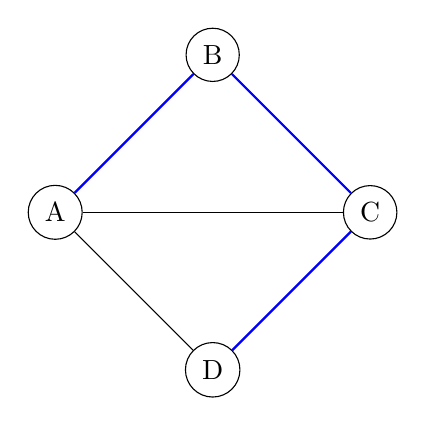
\begin{tikzpicture}
    % Define the vertices
    \node[draw, circle] (A) at (0, 0) {A};
    \node[draw, circle] (B) at (2, 2) {B};
    \node[draw, circle] (C) at (4, 0) {C};
    \node[draw, circle] (D) at (2, -2) {D};
    
    % Define the edges
    \draw (A) -- (B);
    \draw (B) -- (C);
    \draw (C) -- (D);
    \draw (A) -- (C);
    \draw (A) -- (D);
    
    % Highlight the Hamiltonian Path A-B-C-D
    \draw[blue, thick] (A) -- (B);
    \draw[blue, thick] (B) -- (C);
    \draw[blue, thick] (C) -- (D);
\end{tikzpicture}
\end{center}

For the directed graphs below, the graph on the left has a Hamiltonian Path from A to D, while the graph on the right does not have a Hamiltonian Path from A to D.

\begin{center}
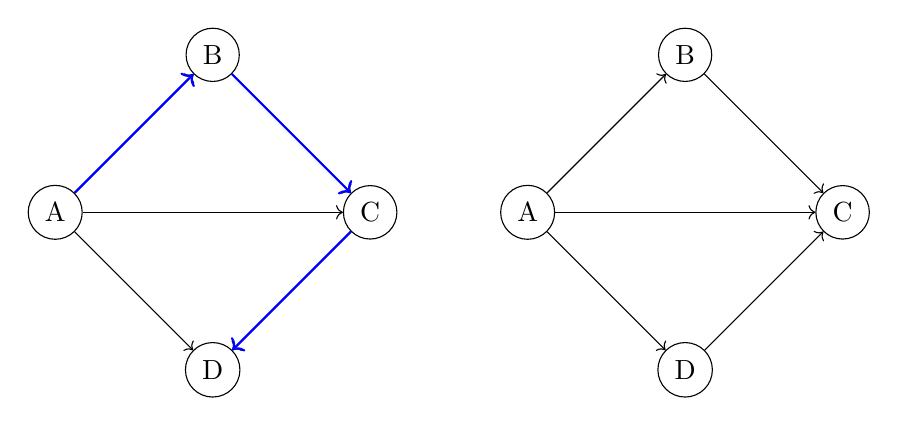
\begin{tikzpicture}
    % First graph with Hamiltonian Path
    \node[draw, circle] (A1) at (0, 0) {A};
    \node[draw, circle] (B1) at (2, 2) {B};
    \node[draw, circle] (C1) at (4, 0) {C};
    \node[draw, circle] (D1) at (2, -2) {D};
    
    \draw[->] (A1) -- (B1);
    \draw[->] (B1) -- (C1);
    \draw[->] (C1) -- (D1);
    \draw[->] (A1) -- (C1);
    \draw[->] (A1) -- (D1);
    
    \draw[blue, thick, ->] (A1) -- (B1);
    \draw[blue, thick, ->] (B1) -- (C1);
    \draw[blue, thick, ->] (C1) -- (D1);

    % Second graph without Hamiltonian Path
    \node[draw, circle] (A2) at (6, 0) {A};
    \node[draw, circle] (B2) at (8, 2) {B};
    \node[draw, circle] (C2) at (10, 0) {C};
    \node[draw, circle] (D2) at (8, -2) {D};
    
    \draw[->] (A2) -- (B2);
    \draw[->] (B2) -- (C2);
    \draw[->] (D2) -- (C2);
    \draw[->] (A2) -- (C2);
    \draw[->] (A2) -- (D2);

\end{tikzpicture}
\end{center}

We refer to the undirected version of this problem as \textbf{UHP} and the directed version as \textbf{DHP}.

\begin{questions}

    \question[3] Give a reduction from UHP to DHP.

    \question[4] Prove the correctness of your reduction from UHP to DHP. That is, prove that the answer to your reduced DHP instance is YES if and only if the answer to UHP is YES. 

    \question[7] Give a reduction from DHP to UHP. You \textbf{do not} need to prove the correctness of this reduction, but you should clearly explain the key components of your reduction and why they are there.

\end{questions}

\clearpage

%===============================
\section{Strategically Placed Krispy Kremes}

This SPKK problem is also in Tutorial 6. UBC Rec student leaders are planning their next fundraiser, and are seeking your help in identifying strategic locations to set up their stands of Krispy Kremes. They have a map showing $n$ locations of buildings and outdoor spots on campus. Their $k$ stands need to be set up in the outdoor spots. They want you to select $k$ spots such that the maximum distance from any of the $n$ locations to a stand is as small as possible.

An instance of the Strategically Placed Krispy Kremes decision problem (SPKK) has a set $V$ of size $n$, a subset $S$ of $V$, an integer $k$, $1\le k \le |S|$,  and a symmetric matrix $d[1..n][1..n]$, plus an additional nonnegative integer $b$. The problem is to determine if there is a subset $S' \subseteq S$ of size $k$, such that

\[
\max_{v \in V} \min_{s \in S'} \{ d[v][s] \;|\; s \in S' \} \le b.
\]

\begin{questions}
\question[8]
Provide a reduction from the Dominating Set problem to SPKK.
Briefly justify why the reduction is polynomial-time (one sentence is sufficient). Carefully explain why your reduction is correct (two paragraphs is sufficient).

  \end{questions}
  
  \clearpage
  
  \section{Very Special Problems}

In this question, we consider special cases of NP-complete problems. Formally, we say that Problem B is a \textbf{special case} of Problem A if every instance of Problem B can be viewed as an instance of Problem A. We've seen examples of this in class: for example, 3-SAT is a special case of SAT (where every clause has length 3). Minimum spanning tree is a special case of Steiner Tree, in which the set of vertices we need to connect includes all the vertices in $V$.

\begin{questions}

\question[4] Consider the \textbf{Bounded-Leaf Spanning Tree Problem (BLST)}: given a graph $G = (V,E)$ and an integer $k$, does $G$ have a spanning tree with no more than $k$ leaves?

Give an NP-complete problem that is a special case of BLST, and justify why this problem is a special case.

\question[3] You showed in the previous question that there is an NP-complete problem that is a special case of BLST, and it is not difficult to show that BLST is in NP (though we are not asking you to do this). Does this imply that BLST is NP-complete? Justify your answer.

\question[4] Give an example of a polytime-solvable problem you have seen in this class that is a special case of an NP-complete problem. Justify your answer.

\end{questions}
  
\end{document}